
  En esta sección veremos un caso de estudio usado para verificar la
implementación.

\section {Problema}

\section {Solución}

\begin{verbatim}
distance :: Event Number
color_r :: Event Number
color_l :: Event Number

type Status = Following, 

delivery = {
  speed_l = 0,
  speed_r = 0,
  faltan_casas

rises :: Event Number -> Event Number
rises = lift fst $ foldE (\(_, last) new -> if last < new then (1, new) else (0, new)) (0,0)

main = let viendo_casa = mapE (hay_casa) distance,
           nueva_casa = rises viendo_casa,
           cuenta = foldE (+) 0 nueva_casa,
           llegue = mapE (>= CASA_ENTREGAR) cuenta,

\end{verbatim}

Se puede ver gráficamente cómo se combinan los eventos, para lograr
con un sensor de distancia y dos sensores de color, definir la velocidad
de los motores, para que nuestro robot se dirija hasta la quinta casa en
su camino.

\begin{figure}[hbtp]
\begin{center}
\caption{Diagrama del caso de estudio}
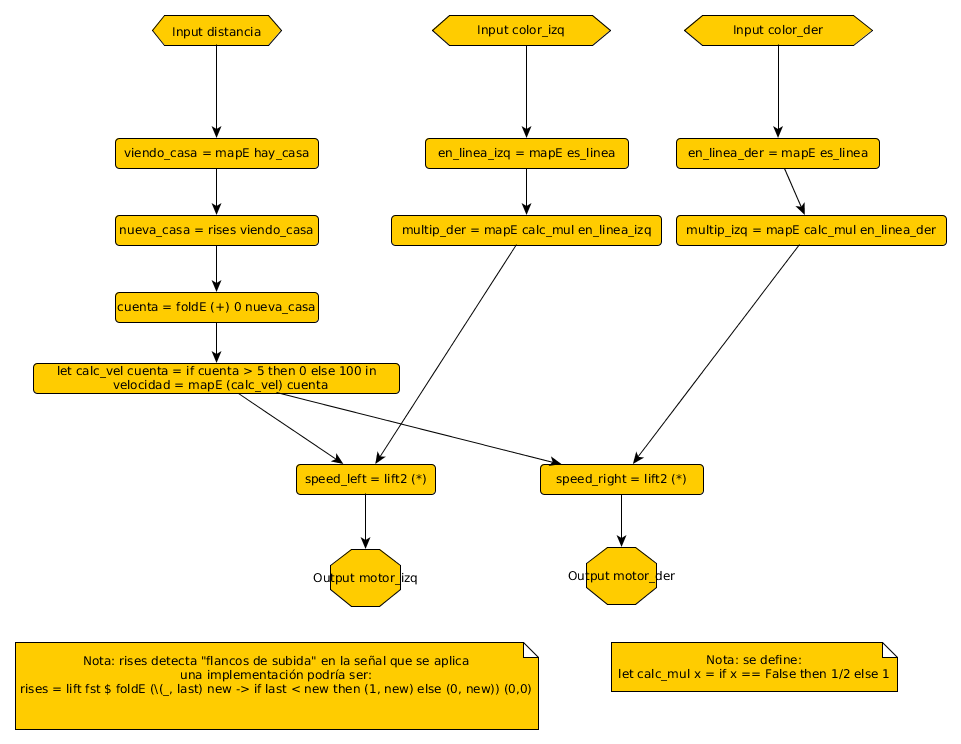
\includegraphics[width=0.9\textwidth]{graphs/delivery.png}
\label{fig:delivery}
\end{center}
\end{figure}


\section {Conclusiones del caso}


